\begin{tcolorbox}[posterbox]
\SectionTitle{Key Findings}
\SmallText
\begin{itemize}
  \item Active numerosity monitoring recruits a frontal \textbf{MMN} (100--120~ms) absent in passive paradigms---indexing automatic change detection.
  \item \textbf{Decreasing} changes yield higher accuracy and \textbf{stronger, later MMN} than Increasing changes.
  \item Neural signals (MMN, N1) \textbf{scale with numerical distance}, mirroring behavioral RT and accuracy.
  \item \textbf{Frontal/posterior dissociation:} Decreasing $>$ Increasing for frontal MMN; Increasing $>$ Decreasing for posterior N1.
\end{itemize}
\end{tcolorbox}

\vspace{0.06in}

\begin{tcolorbox}[posterbox]
\SectionTitle{Theoretical Overview}
\SmallText
\begin{itemize}
  \item \textbf{Dual Systems of Number:} Parallel Individuation (PI) supports small sets (1--3); the Approximate Number System (ANS) handles larger sets (4+).
  \item \textbf{The Gap:} Hyde \& Spelke (2012) demonstrated N1 scaling in passive tasks. Neural mechanisms of \textit{active} numerical change detection---especially direction and distance---remain underexplored.
  \item \textbf{Current Study:} An active ``oddball'' paradigm enables analysis of frontal MMN (automatic change detection) alongside posterior N1 (sensory encoding) and P3b (working memory updating).
\end{itemize}
\end{tcolorbox}

\vspace{0.06in}

\begin{tcolorbox}[posterbox]
\SectionTitle{Experimental Design}
\SmallText
\textbf{Paradigm: Active Change Detection}

Participants monitored streams of dot arrays and pressed a key upon detecting a numerosity change. Feedback and rewards maintained engagement and vigilance.
\begin{itemize}
  \item \textbf{Participants \& Stimuli:} $N=24$ right-handed adults; arrays of 1--6 dots (cumulative area/luminance controlled).
  \item \textbf{Timing:} 250 ms stimulus duration; 750--1250 ms jittered ISI.
  \item \textbf{Habituation:} 3--5 repeats of a prime numerosity.
  \item \textbf{Target:} \textit{No Change} ($3{\rightarrow}3$), \textit{Within-Range} (Small or Large sets), or \textit{Crossover} ($3{\rightarrow}4$, crossing the small/large boundary).
\end{itemize}

\begin{center}
  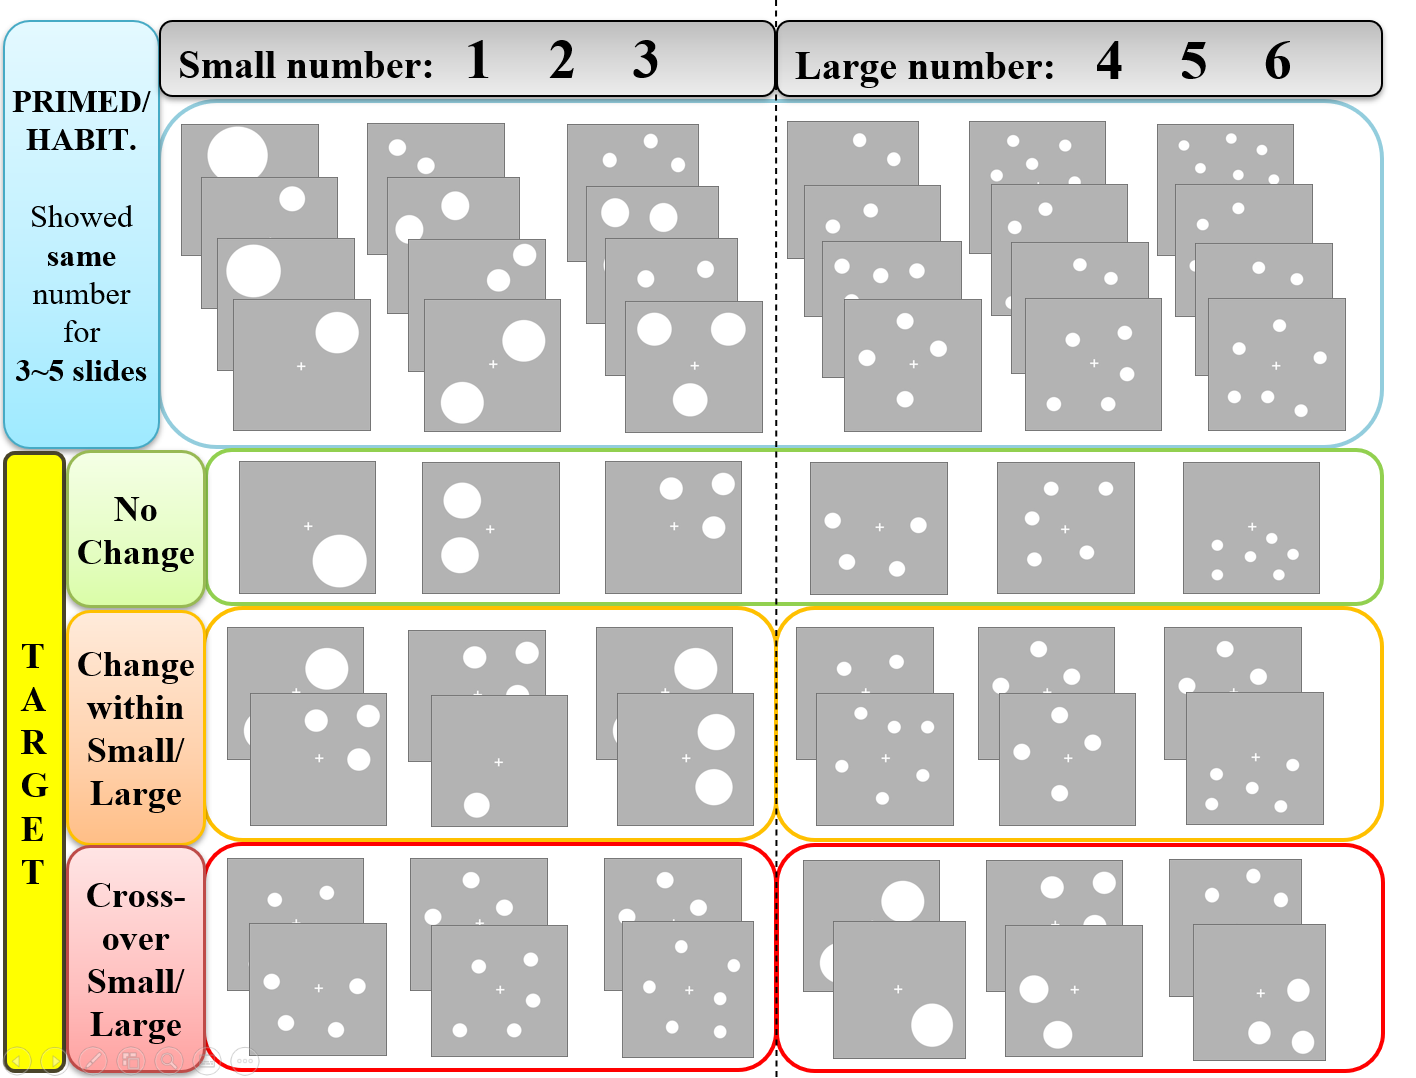
\includegraphics[width=0.66\linewidth, height=10in, keepaspectratio]{media/stimuli_presentation.png}
\end{center}
\SmallText
\textbf{Fig. 1.} Active change-detection task and trial structure.
\end{tcolorbox}

\vfill

\begin{tcolorbox}[posterbox]
\SectionTitle{Acknowledgments}
\SmallText
The authors thank all participants for their contributions. Research was conducted at the Cognition and Language Laboratory, Teachers College, Columbia University. We thank Dr.\ Jean Ee Tang for foundational data collection and prior analysis.
\end{tcolorbox}
